 \documentclass[conference]{IEEEtran}
\usepackage[utf8]{inputenc}
\usepackage{textcomp}
\usepackage[spanish, english]{babel}
\usepackage{amsmath}
\usepackage{amsfonts}
\usepackage{amssymb}
%Dependencies for [1.]
\usepackage{enumerate}
%Dependencies for [1.]
\usepackage{graphicx}
%\usepackage{xcolor}
% Dependencies for Excel2Latex
\usepackage[table]{xcolor}
\usepackage{booktabs}
% Dependencies for Excel2Latex
\usepackage{listings}
\usepackage{tikz}
\usepackage{float}
\usepackage{karnaugh-map}
\usepackage{adjustbox}
\usepackage[left=1cm,right=1cm,top=1cm,bottom=1cm]{geometry}

% Dependencies to reduce size tables
\usepackage{adjustbox}
% Dependencies to reduce size tables

% Command to enable keywords EN
\providecommand{\keywordsen}[1]{\textbf{\textit{Keywords---}} #1}

% Command to enable keywords ES
\providecommand{\keywordses}[1]{\textbf{\textit{Palabras clave---}} #1}

%Habilita bookmarks en PDF
\newcommand\MYhyperrefoptions{bookmarks=true,bookmarksnumbered=true,
pdfpagemode={UseOutlines},plainpages=false,pdfpagelabels=true,
colorlinks=true,linkcolor={black},citecolor={black},
urlcolor={blue}}
\usepackage[\MYhyperrefoptions]{hyperref}
%Habilita bookmarks en PDF

% Dependencies for code blocks
% More info in https://en.wikibooks.org/wiki/LaTeX/Source_Code_Listings
\usepackage{listings}

\lstdefinestyle{CMD_small}
{
    backgroundcolor=\color{black},
    basicstyle=\tiny\color{white}\ttfamily,
    breaklines=true,
    postbreak=\mbox{\textcolor{red}{$\hookrightarrow$}\space},
    keywordstyle=\textcolor{red},
    morekeywords={pip, echo, if, ERRORLEVEL}
}

% Dependencies for code blocks

%Titulo del documento
\title{Proyecto Final de Investigación: Avance 1}

\makeatletter
\newcommand{\linebreakand}{%
  \end{@IEEEauthorhalign}
  \hfill\mbox{}\par
  \mbox{}\hfill\begin{@IEEEauthorhalign} \hfill
}
\makeatother

\renewcommand\thesection{\arabic{section}}
\renewcommand\thesubsection{\thesection.\arabic{subsection}}
\renewcommand\thesubsubsection{\thesubsection.\arabic{subsubsection}}

\author{
	\IEEEauthorblockN{Chavarria Peña Jonathan Andrés}
	\IEEEauthorblockA{\textit{Estudiante Ing. en Sistemas de Computación}\\ 
	\textit{Universidad Fidélitas}\\
	San José, Costa Rica \\
	\href{mailto:jonach1998@gmail.com}{jonach1998@gmail.com}}
\and
	\IEEEauthorblockN{Morales Cordero Valeria}
	\IEEEauthorblockA{\textit{Estudiante Ing. en Sistemas de Computación}\\ 
	\textit{Universidad Fidélitas}\\
	San José, Costa Rica \\
	\href{mailto:valemc0603@gmail.com}{valemc0603@gmail.com}}
\linebreakand % <------------- \and with a line-break
	\IEEEauthorblockN{Phillips Tencio Edmond\hfill}
	\IEEEauthorblockA{\textit{Estudiante Ing. en Sistemas de Computación}\\
	\textit{Universidad Fidélitas}\\
	Alajuela, Costa Rica \\
	\href{mailto:ephillips10986@ufide.ac}{ephillips10986@ufide.ac}}
\and
	\IEEEauthorblockN{Sánchez Camacho Carlos Daniel} 
	\IEEEauthorblockA{\textit{Estudiante Ing. en Sistemas de Computación}\\
	\textit{Universidad Fidélitas}\\
	San José, Costa Rica \\
	\href{mailto:csanchez20965@ufide.ac}{csanchez20965@ufide.ac}}

}


%Inicio del documento
\begin{document}

\maketitle

%Agrega numeracion a las paginas
%\thispagestyle{plain}
%\pagestyle{plain}

\selectlanguage{spanish}

\begin{abstract}
En el presente trabajo de investigación se explicará qué son las pruebas unitarias, para qué se utilizan, como se implementan en las empresas y la manera de generarlas. Para lograrlo se utilizara el lenguaje de programación Python y se le realizaran las pruebas unitarias a un programa que proporciona la información de cada votante incluido en el padrón electoral y los candidatos presidenciales.
\end{abstract}

\selectlanguage{english}
\begin{abstract}
This research will explain what unit tests are, what they are used for, how they are implemented in companies and how to generate them. To achieve this, the Python programming language will be used and the unit tests will be carried out on a program that provides the information of each voter included in the electoral roll and the presidential candidates.
\end{abstract}

\keywordsen{Test, Fail, Priority, Result}

\keywordses{Prueba, Fallo, Prioridad, Resultado}

\section{Investigación de la tecnología}

\subsection{Unit Testing}

En el siguiente proyecto se realizarán pruebas a un programa, las mismas se harán utilizando unit testing; pero para poder utilizarlo es importante comprender qué es y cómo utilizarlo. El unit test se define, como el código necesario para comprobar que el código del programa principal esté funcionando como esperábamos. Los unit test son una de muchas pruebas que se pueden realizar para comprobar que los programas estén en funcionamiento.
Los unit test se conforman de pequeños tests que comprueban que cada parte de los requisitos del código estén correctos; asimismo, se verifican sus resultados.
A la hora de realizar un unit test se puede dividir por partes especificas (Organizar, actuar y afirmar) cada “función” o “caso” que se va a realizar, estas son las siguiente:

\begin{itemize}
\item Arrange: Esta primera parte del caso a testear es donde se deben definir las variables o requisitos que necesita el programa para funcionar.
\item Act: Esta parte consiste en llamar a los métodos o funciones que se desean probar del código del programa principal a testear. 
\item Asert: En la última sección se prueba si los resultados son correctos o incorrectos. Dependiendo del resultado, si son correctos se valida y continúa con los otros casos, o se repara, no se continua hasta que el error desaparezca.
\end{itemize}

Estas partes pueden cambiar de nombre dependiendo de donde se investigue, otros nombres que reciben son Given, When, Then (Dado que, cuando, entonces).
Para la última parte del caso (Asert o Then), si hay errores de integración es necesario investigar si se necesitan otros tipos de pruebas de software y de esta manera lograr comprobar la efectividad total del código.
Al hacer unit testing se asegura que cada parte el código esta bien y es útil. Es importante saber que los fallos y errores son inevitables, por esto mismo los unit test no se pueden considerar como opcionales. Ya que una aplicación, sitio web, programa o código sin pruebas se puede considerar como inestable, voluble o deficiente.
Las pruebas pueden ser desarrolladas por los desarrolladores, mismos que conocen bien el código o también en muchas empresas también las pueden realizar los responsables de QA.

\section{Software a utilizar}

El software a utilizar en la presente investigación es Python -m unittest, es el módulo unittest, este ofrece la posibilidad de crear las pruebas implementando una clase llamada unittest.TestCase en la que se incluirán métodos de pruebas. Tales como los siguientes: 

El modulo de unit test de python permite utilizar distintos contenedores al realizar pruebas unitarias, como por ejemplo: list, dict y set.

Cada una de las pruebas puede devolver tres respuestas dependiendo del resultado, así como las siguientes:

\begin{itemize}
\item OK: Para mostrar que la prueba se ha completado con éxito.
\item FAIL: Para mostrar que la prueba no ha pasado exitosamente y se lanza una excepción como esta: AssertionError (sentencia verdadero-falso)
\item ERROR: Para dar a entender que la prueba no ha pasado exitosamente, pero el resultado en lugar de ser una aserción es un error.
\end{itemize}

Unittest.TestCase este incluye la cantidad de tiempo que tomaron las pruebas, junto con un indicador de estado para cada prueba. 

\subsection{Escritura de pruebas unitarias para el paquete test}

Se prefiere que las pruebas que utilizan el módulo unittest sigan algunas pautas. Una es nombrar el módulo de prueba comenzando con test y terminarlo con el nombre del módulo que se está probando. Los métodos de prueba en el módulo de prueba deben comenzar con test y terminar con una descripción de lo que el método está probando. Esto es necesario para que el controlador de prueba reconozca los métodos como métodos de prueba. Por lo tanto, no se debe incluir una cadena de caracteres de documentación para el método. Se debe usar un comentario (como Tests function returns only True or False) para proporcionar documentación para los métodos de prueba. Esto se hace porque las cadenas de documentación se imprimen si existen y, por lo tanto, no se indica qué prueba se está ejecutando.

\subsection{Plantilla básica para realizar unit test}

\begin{lstlisting}[language=Python,basicstyle=\scriptsize, breaklines=true,
    postbreak=\mbox{\textcolor{red}{$\hookrightarrow$}\space}]
import unittest
from test import support

class MyTestCase1(unittest.TestCase):

    # Only use setUp() and tearDown() if necessary

    def setUp(self):
        ... code to execute in preparation for tests ...

    def tearDown(self):
        ... code to execute to clean up after tests ...

    def test_feature_one(self):
        # Test feature one.
        ... testing code ...

    def test_feature_two(self):
        # Test feature two.
        ... testing code ...

    ... more test methods ...

class MyTestCase2(unittest.TestCase):
    ... same structure as MyTestCase1 ...

... more test classes ...

if __name__ == '__main__':
    unittest.main()

\end{lstlisting}


\section{Programa a probar}

El código al que se le realizarán pruebas será desarrollado en Python, este programa solicita al usuario que ingrese la cédula de la persona que desea buscar y la fecha de nacimiento de la misma, esta información se utilizará para encontrar los datos de la persona en una base de datos ya establecida. Al encontrar la información se imprime en pantalla la siguiente información: saludo, nombre completo, edad, centro de votación y los candidatos oficiales a presidencia y los posibles candidatos. Siendo esta ultima información recolectada desde Wikipedia. La base de datos estará ubicada en el mismo directorio raíz donde esta el programa, si este se borra o se le modifica el nombre, el programa no funcionará.

La idea de este programa es lograr proporcionar de manera fácil información para los votantes. Ya que fácilmente pueden conocer en que región deben votar y los actuales candidatos, además de posibles candidatos a presidencia.


\begin{lstlisting}[style=CMD_small]
C:\Python39\python.exe C:/git/calidad_software_proyecto/Proyecto_Final/Codigo/Votaciones.py
Favor ingrese su cedula sin guiones y con los 0 respectivos: 117110446
Favor ingresar su fecha de nacimiento en el formato dd/mm/yyyy: 13/06/1998
Hola JONATHAN ANDRES
Su nombre completo es: JONATHAN ANDRES CHAVARRIA PENA
Su edad es: 23
Su centro de votacion se ubica en:
	Provincia: SAN JOSE
	Canton: MONTES DE OCA
	Distrito: LOURDES
La lista de candidatos es la siguiente:
                       Partido                  Candidato    Tipo de candidato
0          Liberacion Nacional  Jose Maria Figueres Olsen    Candidato Oficial
1              Nueva Republica    Fabricio Alvarado Munoz    Candidato Oficial
3  Accesibilidad Sin Exclusion   oscar Andres Lopez Arias    Candidato Oficial
4             Accion Ciudadana   Marcia Gonzalez Aguiluz   **Posible Candidato
5             Accion Ciudadana  Carolina Hidalgo Herrera   **Posible Candidato
6             Accion Ciudadana     Welmer Ramos Gonzalez   **Posible Candidato
7             Accion Ciudadana     Hernan Solano Venegas   **Posible Candidato
8             Accion Ciudadana     Martha Zamora Castillo  **Posible Candidato
9        Movimiento Libertario    Carlos Valenciano Kamer    Candidato Oficial

Process finished with exit code 0
\end{lstlisting}

%\begin{figure}[H]
%\centering
%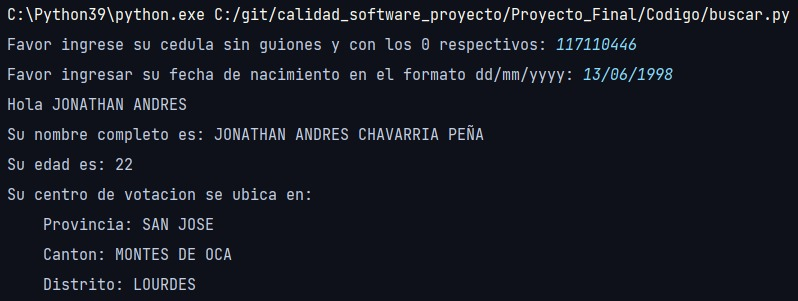
\includegraphics[scale=0.35]{imagenes/ejemplo_programa_a_probar.jpeg}
%\caption{Ejemplo de impresión del programa a probar.}
%\end{figure}


\section{Pruebas a realizar}

Para el proyecto necesitamos saber los casos específicos que vamos a probar en nuestro software por lo que definimos los siguientes:

\begin{enumerate}

\item Probar el caso en el que todo salga bien

\item Probar si la base de datos "Distelec.txt" tiene un formato incorrecto

\item Probar si la base de datos "PADRON\_COMPLETO.txt" tiene un formato incorrecto

\item Probar si se ingresa la cédula con letras o caracteres especiales.

\item Probar si no se encuentra una cedula en la base de datos

\item Probar si se deja alguno de los datos solicitados en blanco

\item Probar si no existe el archivo de la base de datos "Distelec.txt"

\item Probar si no existe el archivo de la base de datos "PADRON\_COMPLETO.txt"

\item Probar si la edad se ingreso en el formato correcto (prueba puede ser: mm/dd/yyyy)

\item Probar si la edad contiene letras o caracteres especiales

\item Probar si la pagina es incorrecta 

\item Probar si la pagina no se encuentra

\end{enumerate}

\section{Plan de pruebas}

\begin{adjustbox}{width=0.5\textwidth}
\begin{tabular}{|c|c|c|}
\hline 
\multicolumn{2}{|c|}{Requerimientos de desarrollo} & \begin{tabular}[c]{@{}l@{}}
• Modulo unittest de Python\\
• Pycharm
\end{tabular} \\
\hline 
\multicolumn{2}{|c|}{Funcionalidades nuevas} & No hay funcionalidades nuevas \\ 
\hline 
\multicolumn{2}{|c|}{Funcionalidades existentes} & \begin{tabular}[c]{@{}l@{}}
• Mostrar datos del usuario incluyendo nombre, apellidos, edad y centro de votación\\
• Mostrar lista de actuales candidatos a presidencia con su partido respectivo\\
\end{tabular} \\
\hline 
\multicolumn{2}{|c|}{Estrategia de pruebas} & \begin{tabular}[c]{@{}l@{}}
Verificar el resultado de cada prueba con lo esperado: \\
\indent • Si el caso pasa la prueba \\
\indent • Si falla por una excepción esperada\\ 
\indent • Si devuelve valores incorrectos\\ 
\end{tabular} \\

\hline 
\multicolumn{2}{|c|}{Pruebas funcionales} & \begin{tabular}[c]{@{}l@{}}
• Todo sale bien\\
• Cédula con letras o caracteres especiales \\
• Fecha nacimiento vacía\\ 
• Formato fecha nacimiento incorrecto\\ 
• Fecha nacimiento caracteres especiales no esperados\\  
\end{tabular} \\
\hline 
\multicolumn{2}{|c|}{Pruebas no funcionales} & \begin{tabular}[c]{@{}l@{}}
• ``Distelec.txt" formato incorrecto\\
• ``PADRON COMPLETO.txt" formato incorrecto\\
• Cédula no encontrada\\
• ``Distelec.txt" no existe\\ 
• ``PADRON COMPLETO.txt" no existe\\ 
• Pagina incorrecta\\ 
• Pagina no existe\\ 
\end{tabular} \\
\hline 
Criterios de inicio & Criterios de suspensión & Criterios de aceptación \\ 
\hline 
\begin{tabular}[c]{@{}l@{}}
El codigo del producto\\
debe de estar listo \\ 
(Producto final para producción)
\end{tabular}
 & 
\begin{tabular}[c]{@{}l@{}}
Se suspende si el tipo de fallo \\ no coincide con el esperado\\
\end{tabular} 
& \begin{tabular}[c]{@{}l@{}}
Se considera aceptado si el 100\% de los unit test tienen PASS. \\Si existen tests que fallaban, y ya no fallan, se consideran también \\ como aceptados, pero se debe modificar el unit test para que ya no falle\\
\end{tabular} \\
\hline 
\multicolumn{2}{|c|}{Entornos y ambientes} & \begin{tabular}[c]{@{}l@{}}
• Python\\
• Pycharm
\end{tabular} \\
\hline 
%\multicolumn{2}{|c|}{Necesidades} & • \\ 
%\hline 
\end{tabular} 
\end{adjustbox}

\section{Casos de prueba}
\subsection{Pruebas Funcionales}
\subsection*{Caso 1}
\begin{itemize}
\item Nombre/Identificador: Todo sale bien.
\item Descripción: El usuario digita bien toda la información.
\item Objetivo de la prueba: Comprobar el buen funcionamiento del programa.
\item Requerimientos o pre condiciones: Estar incluido en la lista de votantes del país.
\item Pasos a seguir: 
\begin{enumerate}
\item Escribir la cédula, en el espacio correspondiente.
\item Escribir la fecha de nacimiento, en el espacio correspondiente.
\end{enumerate}
\item Resultados esperados: Despliegue de toda la información solicitada correcta.
\item Prioridad: Alta.
\end{itemize}
\subsection*{Caso 2}
\begin{itemize}
\item Nombre/Identificador: Cédula con letras o caracteres especiales.
\item Descripción: El usuario digita la cédula utilizando letras o caracteres especiales.
\item Objetivo de la prueba: No poder correr el programa.
\item Requerimientos o pre condiciones: No hay.
\item Pasos a seguir: 
\begin{enumerate}
\item Escribir la cédula conteniendo letras o caracteres especiales, en el espacio correspondiente.
\end{enumerate}
\item Resultados esperados: El programa deja de funcionar y se cierra abruptamente, se quiebra. Exception: KeyError.
\item Prioridad: Alta
\end{itemize}
\subsection*{Caso 3}
\begin{itemize}
\item Nombre: Fecha nacimiento vacío. 
\item Descripción: Probar si se deja alguno de los datos solicitados en blanco.
\item Objetivo de la prueba: Ver el resultado si se deja uno de los datos solicitados en blanco. 
\item Requerimientos: Base de datos. 
\item Pasos a seguir:
\begin{enumerate}
\item Ingresar los datos y probar dejando algunos espacios en blanco para ver el resultado
\end{enumerate}
\item Resultados esperados: El programa deja de funcionar y se cierra abruptamente, se quiebra. Exception: ValueError.
\item Prioridad: Alta.
\end{itemize}
\subsection*{Caso 4}
\begin{itemize}
\item Nombre: Formato fecha nacimiento incorrecto. 
\item Descripción: Probar si la edad se ingresó en el formato incorrecto.
\item Objetivo de la prueba: verificar que la edad no se ingreso en el formato deseado. 
\item Requerimientos: Ingresar fecha de nacimiento, base de datos. 
\item Pasos por seguir: 
\begin{enumerate}
\item Ingresar la fecha de nacimiento en formato incorrecto.
\end{enumerate}
\item Resultados esperados: El programa continua, finaliza, sin embargo, despliega la edad incorrecta.
\item Prioridad: Alta.
\end{itemize}

\subsection*{Caso 5}
\begin{itemize}
\item Nombre: Fecha nacimiento caracteres especiales no esperados.
\item Descripción: \item Probar si la edad contiene letras o caracteres especiales.
\item Objetivo de la prueba: Ver que sucede si se ingresa la edad con caracteres no esperados por el programa (letras o caracteres especiales) datos.
\item Requerimientos: Ingresar la edad. 
\item Pasos por seguir: 
\begin{enumerate}
\item Ingresar la edad en el sistema con letras o caracteres especiales y comprobar que sucede.
\end{enumerate}
\item Resultados esperados: El programa deja de funcionar y se cierra abruptamente, se quiebra. Exception: ValueError.
\item Prioridad: Media
\end{itemize}
\subsection{Pruebas No Funcionales}
\subsection*{Caso 1}
\begin{itemize}
\item Nombre/Identificador: ``Distelec.txt" formato incorrecto.
\item Descripción: Verificar que el archivo Distelec este separado por otro carácter que no sea comas.
\item Objetivo de la prueba: Comprobar que el programa falle cuando el archivo no esta separado por comas. 
\item Requerimientos o pre condiciones: Archivo en el formato incorrecto.
\item Pasos a seguir: 
\begin{enumerate}
\item Buscar el archivo ``Distelec.txt" en la carpeta donde esta el programa.
\item Separar la información del archivo, utilizando como referencia la "," para separar.
\end{enumerate}
\item Resultados esperados: El programa deja de funcionar y se cierra abruptamente, se quiebra. Exception: KeyError.
\item Prioridad: Alta
\end{itemize}

\subsection*{Caso 2}
\begin{itemize}
\item Nombre/Identificador: ``PADRON\_COMPLETO.txt" formato incorrecto.
\item Descripción: Verificar que el archivo PADRON\_COMPLETO este separado por otro carácter que no sea comas.
\item Objetivo de la prueba: Comprobar que el programa falle cuando el archivo no esta separado por comas. 
\item Requerimientos o pre condiciones: Archivo en el formato incorrecto.
\item Pasos a seguir: 
\begin{enumerate}
\item Buscar el archivo ``PADRON\_COMPLETO.txt" en la carpeta donde esta el programa.
\item Separar la información del archivo, utilizando como referencia la "," para separar.
\end{enumerate}
\item Resultados esperados: El programa deja de funcionar y se cierra abruptamente, se quiebra. Exception: ValueError.
\item Prioridad: Alta
\end{itemize}



\subsection*{Caso 3}
\begin{itemize}
\item Nombre: Cédula no encontrada.
\item Descripción: Probar si no se encuentra una cédula en la base de datos.
\item Objetivo de la prueba: Identificar que sucede si no se encuentra una cédula ingresada.
\item Requerimientos: Ingresar una cédula, base de datos. 
\item Pasos para seguir: 
\begin{enumerate}
\item Ingresar una cédula en el campo correspondiente y ver el resultado. 
\end{enumerate}
\item Resultados esperados: El programa deja de funcionar y se cierra abruptamente, se quiebra. Exception: KeyError.
\item Prioridad: Alta.

\end{itemize}



\subsection*{Caso 4}
\begin{itemize}
\item Nombre: ``Distelec.txt"  no existe. 
\item Descripción: Probar si no existe el archivo de la base de datos ``Distelec.txt".
\item Objetivo de la prueba: Ver si no existe el archivo "Distelec.txt" de la base de datos que sucede con el programa.
\item Requerimientos: Documento "Distelec.txt".
\item Pasos a seguir: 
\begin{enumerate}
\item Verificar la existencia o no del archivo "Distelec.txt" en la base de datos y ejecutar el programa. 
\end{enumerate} 
\item Resultados esperados: El programa deja de funcionar y se cierra abruptamente, se quiebra. Exception: FileNotFoundError.
\item Prioridad: Muy alta.
\end{itemize}

\subsection*{Caso 5}
\begin{itemize}
\item Nombre: ``PADRON\_COMPLETO.txt"  no existe.
\item Descripción: Probar si no existe el archivo de la base de datos ``PADRON\_COMPLETO.txt".
\item Objetivo de la prueba: Verificar lo que sucede si no se encuentra en el programa el archivo de la base de datos ``PADRON\_COMPLETO.txt".
\item Requerimientos: Documento ``PADRON\_COMPLETO.txt".
\item Pasos a seguir:
\begin{enumerate}
\item Ejecutar el programa y ver que sucede si no se encuentra el archivo ``PADRON\_COMPLETO.txt".
\end{enumerate}
\item Resultados esperados: El programa deja de funcionar y se cierra abruptamente, se quiebra. Exception: FileNotFoundError.
\item Prioridad: Muy alta. 
\end{itemize}





\subsection*{Caso 6}
\begin{itemize}
\item Nombre: Página incorrecta
\item Descripción: Probar si la página es incorrecta
\item Objetivo de la prueba: Ver que sucede al ingresar a una página incorrecta.
\item Requerimientos: Página incorrecta.
\item Pasos por seguir: Confirmar que sucede si se ingresa a una pagina incorrecta.
\item Resultados esperados: El programa deja de funcionar y se cierra abruptamente, se quiebra. Exception: IndexError.
\item Prioridad: Muy alta.
\end{itemize}

\subsection*{Caso 7}

\begin{itemize}
\item Nombre: Pagina no existe.
\item Descripción: Probar si la página no se encuentra.
\item Objetivo de la prueba: Verificar lo que sucede si no se encuentra la pagina.
\item Requerimientos: Dirección de página correcta.
\item Pasos por seguir: 
\begin{enumerate}
\item Ejecutar el programa y ver que sucede si no encuentra la dirección de la página correcta.
\end{enumerate}
\item Resultados esperados: El programa deja de funcionar y se cierra abruptamente, se quiebra. Exception: requests.exceptions.MissingSchema.
\item Prioridad: Muy alta. 
\end{itemize}

\section{Pruebas Unitarias}

\begin{lstlisting}[language=Python, basicstyle=\tiny, breaklines=true,
    postbreak=\mbox{\textcolor{red}{$\hookrightarrow$}\space}]
    
class TestVotaciones(unittest.TestCase):
    def setUp(self) -> None:
	self._target = Votaciones("dummy", "dummy", "dummy")
	self._distelec = """101001,SAN JOSE,CENTRAL,HOSPITAL                                                          
	108001,SAN JOSE,CENTRAL,HATILLO"""
	self._padron = """100339724,109007, ,20231119,00000,JOSE,DELGADO,CORRALES         
	100842598,108001, ,20261024,00000,CARMEN                        ,CORRALES                  ,MORALES           
	101019387,101026, ,20230416,00000,CLAUDIA MANUELA               ,ESPINOZA                  ,FONSECA"""
	self._distelec_return = mock.mock_open(read_data=self._distelec).return_value
	self._padron_return = mock.mock_open(read_data=self._padron).return_value
	self._url_return = url

    # Caso 1
    @mock.patch("Proyecto_Final.Codigo.Votaciones.requests")
    @mock.patch("Proyecto_Final.Codigo.Votaciones.input")
    @mock.patch("Proyecto_Final.Codigo.Votaciones.open")
    @mock.patch('sys.stdout', new_callable=io.StringIO)
    def test_todo_sale_bien(self, mock_stdout, mock_open, mock_input, mock_requests):
        mock_open.side_effect = [self._distelec_return, self._padron_return]
        mock_input.side_effect = ["100842598", "13/12/1998"]
        mock_requests.get.return_value.content = url
        self._target.run()
        target_output = mock_stdout.getvalue()
        expected_output = """Hola CARMEN
Su nombre completo es: CARMEN CORRALES MORALES
Su edad es: 22
Su centro de votacion se ubica en:
	Provincia: SAN JOSE
	Canton: CENTRAL
	Distrito: HATILLO
La lista de candidatos es la siguiente:
                        Partido                            Candidato    Tipo de candidato
0           Liberacion Nacional            Jose Maria Figueres Olsen    Candidato Oficial
1               Nueva Republica              Fabricio Alvarado Munoz    Candidato Oficial
2   Progreso Social Democratico                Rodrigo Chaves Robles    Candidato Oficial
3       Unidad Social Cristiana              Lineth Saborio Chaverri    Candidato Oficial
4                Unidos Podemos                Natalia Diaz Quintana    Candidato Oficial
6   Accesibilidad Sin Exclusion             oscar Andres Lopez Arias    Candidato Oficial
7              Accion Ciudadana             Marcia Gonzalez Aguiluz   **Posible Candidato
8              Accion Ciudadana            Carolina Hidalgo Herrera   **Posible Candidato
9              Accion Ciudadana               Welmer Ramos Gonzalez   **Posible Candidato
10             Accion Ciudadana               Hernan Solano Venegas   **Posible Candidato
11        Movimiento Libertario              Carlos Valenciano Kamer    Candidato Oficial
12             Nueva Generacion                     Sergio Mena Diaz    Candidato Oficial
13                Union Liberal             Federico Malavassi Calvo    Candidato Oficial
14                  Por definir          Juan Diego Castro Fernandez  **Posible Candidato
15                  Por definir                       Viviam Quesada  **Posible Candidato
17     Coalicion para el Cambio               Eliecer Feinzaig Mintz    Candidato Oficial
18                Frente Amplio  Jose Maria Villalta Florez-Estrada     Candidato Oficial
19        Restauracion Nacional                 Eduardo Cruickshank   **Posible Candidato
20        Restauracion Nacional                        Melvin Nunez   **Posible Candidato
"""
        self.assertEqual(expected_output, target_output)

    # Caso 2
    @mock.patch("Proyecto_Final.Codigo.Votaciones.input")
    @mock.patch("Proyecto_Final.Codigo.Votaciones.open")
    def test_distelect_formato_incorrecto(self, mock_open, mock_input):
        distelec = """101001-SAN JOSE-CENTRAL-HOSPITAL
108001-SAN JOSE-CENTRAL-HATILLO"""
        distelec_return = mock.mock_open(read_data=distelec).return_value
        mock_open.side_effect = [distelec_return, self._padron_return]
        mock_input.side_effect = ["100842598", "13/12/1998"]
        with self.assertRaises(KeyError):
            self._target.run()

    # Caso 3
    @mock.patch("Proyecto_Final.Codigo.Votaciones.input")
    @mock.patch("Proyecto_Final.Codigo.Votaciones.open")
    def test_padron_formato_incorrecto(self, mock_open, mock_input):
        padron = """100339724-109007- -20231119-00000-JOSE-DELGADO-CORRALES         
100842598-108001- -20261024-00000-CARMEN                        -CORRALES                  -MORALES           
101019387-101026- -20230416-00000-CLAUDIA MANUELA               -ESPINOZA                  -FONSECA"""
        padron_return = mock.mock_open(read_data=padron).return_value
        mock_open.side_effect = [self._distelec_return, padron_return]
        mock_input.side_effect = ["100842598", "13/12/1998"]
        with self.assertRaises(ValueError):
            self._target.run()

    # Caso 4
    @mock.patch("Proyecto_Final.Codigo.Votaciones.input")
    @mock.patch("Proyecto_Final.Codigo.Votaciones.open")
    def test_cedula_caracteres_especiales_y_letras(self, mock_open, mock_input):
        mock_open.side_effect = [self._distelec_return, self._padron_return]
        mock_input.side_effect = ["holi151.<?", "13/12/1998"]
        with self.assertRaises(KeyError):
            self._target.run()

    # Caso 5
    @mock.patch("Proyecto_Final.Codigo.Votaciones.input")
    @mock.patch("Proyecto_Final.Codigo.Votaciones.open")
    def test_cedula_no_encontrada(self, mock_open, mock_input):
        mock_open.side_effect = [self._distelec_return, self._padron_return]
        mock_input.side_effect = ["117110446", "13/06/1998"]
        with self.assertRaises(KeyError):
            self._target.run()

    # Caso 6
    @mock.patch("Proyecto_Final.Codigo.Votaciones.input")
    @mock.patch("Proyecto_Final.Codigo.Votaciones.open")
    def test_fecha_nacimiento_vacio(self, mock_open, mock_input):
        mock_open.side_effect = [self._distelec_return, self._padron_return]
        mock_input.side_effect = ["100842598", ""]
        with self.assertRaises(ValueError):
            self._target.run()

    # Caso 7
    def test_distelect_no_existe(self):
        with self.assertRaises(FileNotFoundError):
            self._target.run()

    # Caso 8
    def test_padron_no_existe(self):
        target = Votaciones("Database/Distelec.txt", "dummy", "dummy")
        with self.assertRaises(FileNotFoundError):
            target.run()

    # Caso 9
    @mock.patch("Proyecto_Final.Codigo.Votaciones.requests")
    @mock.patch("Proyecto_Final.Codigo.Votaciones.input")
    @mock.patch("Proyecto_Final.Codigo.Votaciones.open")
    @mock.patch('sys.stdout', new_callable=io.StringIO)
    def test_formato_fecha_nacimiento_incorrecto(self, mock_stdout, mock_open, mock_input, mock_requests):
        mock_open.side_effect = [self._distelec_return, self._padron_return]
        mock_input.side_effect = ["100842598", "13/12/98"]
        mock_requests.get.return_value.content = url
        self._target.run()
        target_output = mock_stdout.getvalue()
        expected_output = """Hola CARMEN
Su nombre completo es: CARMEN CORRALES MORALES
Su edad es: 1922
Su centro de votacion se ubica en:
\tProvincia: SAN JOSE
\tCanton: CENTRAL
\tDistrito: HATILLO
La lista de candidatos es la siguiente:
                        Partido                            Candidato    Tipo de candidato
0           Liberacion Nacional            Jose Maria Figueres Olsen    Candidato Oficial
1               Nueva Republica              Fabricio Alvarado Munoz    Candidato Oficial
2   Progreso Social Democratico                Rodrigo Chaves Robles    Candidato Oficial
3       Unidad Social Cristiana              Lineth Saborio Chaverri    Candidato Oficial
4                Unidos Podemos                Natalia Diaz Quintana    Candidato Oficial
6   Accesibilidad Sin Exclusion             oscar Andres Lopez Arias    Candidato Oficial
7              Accion Ciudadana             Marcia Gonzalez Aguiluz   **Posible Candidato
8              Accion Ciudadana            Carolina Hidalgo Herrera   **Posible Candidato
9              Accion Ciudadana               Welmer Ramos Gonzalez   **Posible Candidato
10             Accion Ciudadana               Hernan Solano Venegas   **Posible Candidato
11        Movimiento Libertario              Carlos Valenciano Kamer    Candidato Oficial
12             Nueva Generacion                     Sergio Mena Diaz    Candidato Oficial
13                Union Liberal             Federico Malavassi Calvo    Candidato Oficial
14                  Por definir          Juan Diego Castro Fernandez  **Posible Candidato
15                  Por definir                       Viviam Quesada  **Posible Candidato
17     Coalicion para el Cambio               Eliecer Feinzaig Mintz    Candidato Oficial
18                Frente Amplio  Jose Maria Villalta Florez-Estrada     Candidato Oficial
19        Restauracion Nacional                 Eduardo Cruickshank   **Posible Candidato
20        Restauracion Nacional                        Melvin Nunez   **Posible Candidato
"""
        self.assertEqual(expected_output, target_output)

    # Caso 10
    @mock.patch("Proyecto_Final.Codigo.Votaciones.input")
    @mock.patch("Proyecto_Final.Codigo.Votaciones.open")
    def test_fecha_nacimiento_caracteres_especiales_no_esperados(self, mock_open, mock_input):
        mock_open.side_effect = [self._distelec_return, self._padron_return]
        mock_input.side_effect = ["100842598", "13-12-1998"]
        with self.assertRaises(ValueError):
            self._target.run()

    # Caso 11
    @mock.patch("Proyecto_Final.Codigo.Votaciones.input")
    @mock.patch("Proyecto_Final.Codigo.Votaciones.open")
    def test_pagina_incorrecta(self, mock_open, mock_input):
        target = Votaciones("dummy", "dummy", "https://es.wikipedia.org/wiki/Elecciones_generales_de_Costa_Rica_de_3022")
        mock_open.side_effect = [self._distelec_return, self._padron_return]
        mock_input.side_effect = ["100842598", "13/06/1998"]
        with self.assertRaises(IndexError):
            target.run()

    # Caso 12
    @mock.patch("Proyecto_Final.Codigo.Votaciones.input")
    @mock.patch("Proyecto_Final.Codigo.Votaciones.open")
    def test_pagina_no_existe(self, mock_open, mock_input):
        mock_open.side_effect = [self._distelec_return, self._padron_return]
        mock_input.side_effect = ["100842598", "13/06/1998"]
        with self.assertRaises(requests.exceptions.MissingSchema):
            self._target.run()

\end{lstlisting}

\section{Bug Report}

\subsection*{Bug 1}
\begin{itemize}

\item Título: “Distelec.txt” formato incorrecto.

\item Descripción: Verificar que el archivo Distelec este separado por otro carácter que no sea comas.

\item Resultado esperado: El programa funciona correctamente si se escribe separado con comas.

\item Resultado desplegado: El programa deja de funcionar y se cierra abruptamente, se quiebra. 

\item Pasos por seguir: 
\begin{enumerate}
\item Buscar el archivo “Distelec.txt” en la carpeta donde está el programa.
\item Separar la información del archivo, utilizando como referencia un “.” para separar.
\end{enumerate}

\item Otros datos Relevantes: Exception: KeyError.
\end{itemize}
\subsection*{Bug 2}
\begin{itemize}
\item Título: “PADRON COMPLETO.txt” formato incorrecto.

\item Descripción: Verificar que el archivo PADRON COMPLETO este separado por otro carácter que no sea comas.

\item Resultado esperado: El programa funciona correctamente si se escribe separado con comas.

\item Resultado desplegado: El programa deja de funcionar y se cierra abruptamente, se quiebra.  

\item Pasos por seguir: 
\begin{enumerate}
\item Buscar el archivo “PADRON COMPLETO.txt” en la carpeta donde está el programa.  
\item Separar la información del archivo, utilizando como referencia el ”.” para separar.
\end{enumerate}
\item Otros datos Relevantes: Exception: ValueError.
\end{itemize}
\subsection*{Bug 3}
\begin{itemize}
\item Título: Cedula con letras o caracteres especiales.

\item Descripción: El usuario digita la cedula utilizando letras o caracteres especiales.

\item Resultado esperado: El programa funciona correctamente si se escribe con números.

\item Resultado desplegado: El programa deja de funcionar y se cierra abruptamente, se quiebra. 

\item Pasos por seguir: 
\begin{enumerate}
\item Escribir la cédula conteniendo letras o caracteres especiales en el espacio incorrecto.
\end{enumerate}

\item Otros datos Relevantes: Exception: KeyError.
\end{itemize}
\subsection*{Bug 4}
\begin{itemize}
\item Título: Cédula no encontrada.

\item Descripción: Probar si no se encuentra una cedula en la base de datos.

\item Resultado esperado: El programa encuentra la cedula y continua su ejecución.

\item Resultado desplegado: El programa deja de funcionar y se cierra abruptamente.
 
\item Pasos para seguir: 
\begin{enumerate}
\item Ingresar una cedula incorrecta en el campo correspondiente y ver el resultado.
\end{enumerate}
\item Otros datos Relevantes: Exception: KeyError.

\end{itemize}
\subsection*{Bug 5}
\begin{itemize}
\item Título: Fecha nacimiento vacío.

\item Descripción: Probar si se deja alguno de los datos solicitados en blanco.

\item Resultado esperado: El usuario ingresa todos los datos solicitados.

\item Resultado desplegado: El programa deja de funcionar y se cierra abruptamente, se quiebra. 

\item Pasos por seguir: 
\begin{enumerate}
\item Ingresar los datos y probar dejando algunos espacios en blanco para ver el resultado
\end{enumerate}
\item Otros datos Relevantes: Exception: ValueError.
\end{itemize}
\subsection*{Bug 6}
\begin{itemize}
\item Título: “Distelec.txt” no existe.

\item Descripción: Probar si no existe el archivo de la base de datos ´ “Distelec.txt”.

\item Resultado esperado: El sistema encuentra en la Base de Datos el distelec.txt

\item Resultado desplegado: El programa deja de funcionar y se cierra abruptamente, se quiebra. 

\item Pasos por seguir: 
\begin{enumerate}
\item Verificar la existencia o no del archivo” Distelec.txt” en la base de datos y ejecutar el programa.
\end{enumerate}

\item Otros datos Relevantes: Exception: FileNotFoundError

\end{itemize}
\subsection*{Bug 7}
\begin{itemize}
\item Título: “PADRON COMPLETO.txt” no existe.

\item Descripción: Probar si no existe el archivo de la base de datos ´ “PADRON COMPLETO.txt”

\item Resultado esperado: El sistema encuentra en la Base de Datos el 
Padron.txt.

\item Resultado desplegado: El programa deja de funcionar y se cierra abruptamente, se quiebra. 

\item Pasos por seguir: 
\begin{enumerate}
\item Ejecutar el programa y ver que sucede si no se encuentra el archivo “PADRON COMPLETO.txt”.
\end{enumerate}
\item Otros datos Relevantes: Exception: FileNotFoundError.

\end{itemize}
\subsection*{Bug 8}
\begin{itemize}
\item Título: Formato fecha nacimiento incorrecto.

\item Descripción: Probar si la edad se ingresa en el formato correcto.

\item Resultado esperado: El usuario ingresa la fecha de nacimiento en el formato correcto.

\item Resultado desplegado: El programa continuo, finaliza, sin embargo, despliega la edad incorrecta.

\item Pasos por seguir: 
\begin{enumerate}
\item Ingresar la fecha de nacimiento en formato incorrecto.
\end{enumerate}

\end{itemize}
\subsection*{Bug 9}
\begin{itemize}
\item Título: Fecha nacimiento caracteres especiales no esperados.

\item Descripción: Probar si la edad contiene letras o caracteres especiales.

\item Resultado esperado: El usuario ingresa la Fecha de nacimiento en el formato correcto.

\item Resultado desplegado: El programa deja de funcionar y se cierra abruptamente, se quiebra. 

\item Pasos por seguir: 
\begin{enumerate}
\item Ingresar la edad en el sistema con letras o caracteres especiales y comprobar que sucede.
\end{enumerate}
\item Otros datos Relevantes: Exception: ValueError.
\end{itemize}


\subsection*{Bug 10}
\begin{itemize}
\item Título: Pagina incorrecta

\item Descripción: Probar si la página es incorrecta

\item Resultado esperado: La página es correcta y el sistema sigue.

\item Resultado desplegado: El programa deja de funcionar y se cierra abruptamente, se quiebra. 

\item Pasos por seguir: 
\begin{enumerate}
\item Se ingresa a una página incorrecta.
\end{enumerate}
\item Otros datos Relevantes: Exception: IndexError.
\end{itemize}
\subsection*{Bug 11}
\begin{itemize}
\item Título: Pagina no existe

\item Descripción: Probar si la página no se encuentra.

\item Resultado esperado: EL sistema encuentra la pagina y continua con su ejecución.

\item Resultado desplegado: El programa deja de funcionar y se cierra abruptamente, se quiebra. 

\item Pasos por seguir: 
\begin{enumerate}
\item Ejecutar el programa y ver que sucede si no encuentra la dirección de la página correcta.
\end{enumerate}
\item Otros datos Relevantes: Exception: requests.exceptions.MissingSchema.

\end{itemize}



%\section{Conclusiones}



\normalsize

\begin{thebibliography}{}


\bibitem{Giuseppe_Vetri} \textsc{Giuseppe Vetri} (2020). \textit{Que es un unit test (Prueba unitaria).} \url{https://dev.to/codingpizza/que-es-un-unit-test-prueba-unitaria-2dnk}\\

\bibitem{yeeply} \textsc{Yeeply.} (2021). \textit{¿Qué son las pruebas unitarias y cómo llevar una a cabo?.} \url{https://www.yeeply.com/blog/que-son-pruebas-unitarias/} \\

\bibitem{Unittest} \textsc{Héctor Costa Guzmán} (2018). \textit{Unittest.} \url{https://docs.hektorprofe.net/python/documentacion-y-pruebas/unittest/} \\

\bibitem{m} \textsc{Python Software Foundation} (2018). \textit{Línea de comandos y entorno.} \url{https://docs.python.org/es/3.10/using/cmdline.html#cmdoption-m} \\



\end{thebibliography}


\end{document}
